\section{Fixity Information}
Fixity Information provides the Data integrity checks or validation/verification keys used to ensure that the particular Content Information object has not been altered in an undocumented manner\cite[8]{lee2010open}. In this thesis, fixity information will be a transaction hash, with which the fixity information can be retrieved from the Ethereum blockchain.
With fixity information you are able to answer questions regarding the authenticity and integrity of an object, which supports assertions about the authenticity and trustworthiness of digital objects \cite[3]{ndsa2017fixity}.
\newline \textit{Have you received the files you expected?} When fixity information is provided with objects upfront, it can be used to validate that you have received what was intended for the collection.
\newline \textit{Is the data corrupted or altered from what you expected?}  Once you have generated baseline fixity information for files or objects, comparing that information with future fixity check information will tell you if a file has changed or been corrupted.
\newline \textit{Can you prove you have the data/files you expected, and they are not corrupt or altered?} By providing fixity information alongside content, you enable your users to verify that what they have is identical to what you say it should be. 

Fixity is a key concept for the long-term preservation and management of digital material for many reasons. Previous scholarship on fixity has shown its vital importance in discovering changes to data and all that this error-checking can imply: authenticity and renderability of files, trustworthiness of institutions, and system monitoring/maintenance. Despite the centrality of fixity to the field of digital preservation, there is little prescriptive guidance on when and how to create fixity information, where to store it, and how often to check it. This absence is not without reason, however: the incredible variety of organizational structures, priorities, staffing levels, funding, resources, and size of collections held by institutions that do digital preservation make it difficult to establish a single set of one-size-fits-all best practices \cite[38]{ndsa2017fixity}.
\subsection{Generating Fixity Information on Ingest}
 It is important to check the fixity
of content transferred to you when you bring it under your stewardship. Whenever possible, it is ideal to encourage content providers or producers to submit fixity information along with content objects. You can only provide assurance about the fixity of content overtime once you have initial fixity values, thus it is imperative to document fixity information as soon as possible. If fixity information is not provided as part of the transfer, you should create fixity information once you have received the materials \cite[4]{ndsa2014fixity}.

\subsection{Fixity Checks}
In addition to checking fixity before and after transfer, collections of digital files and objects should be checked on a regular basis. There are a range of systems and approaches focused on checking the fixity values of all objects at regular intervals. This could be monthly, quarterly, or yearly for example. The more often you check, the more likely you are to detect and repair errors \cite[4]{ndsa2014fixity}.
The information must be put to use, in the form of scheduled audits of the objects against the fixity information. Additionally, replacement or repair processes must be in place. Ideally these will have been tested before being needed. All of this is critical for bit-level preservation, but ensuring fixity does not mean that the object is or will be understandable. Long term access is also contingent on ones ability to make sense of and use the contents of the file in the future \cite[2]{ndsa2014fixity}.

Most fixity procedures involve a computational method that takes a digital file as input and outputs an alphanumeric value; this output value is used as a baseline comparison each time the fixity check is rerun \cite[5]{ndsa2017fixity}. 
For example, fixity checks may occur at different times depending on the institution's environment: during initial deposit only; during any file transmission; during scheduled backup routines; or periodically at specified times or when manually triggered \cite[7]{ndsa2017fixity}.\newline The rate of fixity checking is going to be dependent on how quickly you can run the checks, the complexity of your chosen fixity instrument, and how much of your resources (e.g., CPU, memory, bandwidth) can be used for this operation. This can become a choke point as the amount of digital content increases but the infrastructure to perform the checks stays the same. In a situation like this, the fixity checking activities can adversely affect other important functions like delivery of the content to users.
\subsection{Fixity Instruments}
\begin{table}[p]
    \centering
    \caption{Various Fixity Instruments \cite[6]{ndsa2017fixity}}
    \label{tb:fixity-instruments}
    \begin{tabular}{c|p{0.4\textwidth}|p{0.4\textwidth}}
     Fixity Instrument & Definition & Level of Effort and Return of Investment\\
     \hline
     Expected File Size & File size that differs from the expected can be an indicator of problems, for example by highlighting zero byte files & Low level of effort and low level detail. File size is auto-generated technical metadata that can be viewed in Windows Explorer or other common tools. \\  
     \hline
     Expected File Count & File count that differs from the expected can be an indicator that files are either added or dropped from the package. & Low level of effort and low level detail. File count is auto-generated technical metadata that can be viewed in Windows Explorer or other common tools.  \\
     \hline
     CRC & Error detection code, typically used during network transfers. & Low level of effort and moderate level of detail. CRC function values, which are variable but typically 32 or 64 bit, are relatively easy to implement and analyze.  \\
     \hline
     MD5 & Cryptographic hash function & Moderate level of effort and high level of detail. CPU and processing requirements to compute the hash values are low to moderate depending on the size of the file. The output size of this hash value is the lowest of the cryptographic hash values at 128 bits.  \\
     \hline
     SHA1 & Cryptographic hash function & Moderate level of effort, high level of detail, and added security assurance. Due to its higher 160-bit output hash value, SHA-1 requires more relative time to compute for a given number of processing cycles CPU and processing time than MD5.  \\
     \hline
     SHA256 & More secure cryptographic hash function & High level of effort, very high level of detail, and added security assurance. With an output hash value of 256 bits, SHA-256 requires more relative time to compute for a given number of processing cycles CPU and processing time than SHA-1. 
    \end{tabular}
\end{table}
For a given fixity instrument, see Table \ref{tb:fixity-instruments}, the harder it is to find two objects that result in the same fixity information, the more “collision resistant” that instrument is. This is important mostly for preventing the concealment of intentional changes to objects. For example, expected file size and expected file count are extremely vulnerable to collision: it is very easy for someone to replace an object with one that matches in file size. It is also possible (although unlikely) for an unintentional change (such as corruption or human error) to result in an object with the same fixity information for instruments that have low collision resistance. Of the fixity instruments described above, the cryptographic hash functions (MD-5, SHA-1, and SHA-256) are the most collision resistant; SHA-256 is recommended for applications where security is important. However, performing fixity checking and replacing damaged objects is critical for any preservation system, and using any fixity instrument is much better than none at all. Note that as the level of security of the hash function increases, so do the time and resources needed to compute \cite[7]{ndsa2014fixity}.
\subsection{Storage Medium}
\label{sec:storage-medium}
There are various storages to store fixity information, each of them has some advantages and disadvantages in terms of conveniency, security and throughput.
\newline \textit{In object metadata records:} In many cases, you will want to record some file or object fixity information wherever you store and manage the metadata records. These metadata records are actually stored as discrete files or in databases. This is particularly useful for maintaining originally submitted or generated fixity information as part of the long-term object metadata. 
\newline \textit{In databases and logs:} For checks you run at given intervals you may not want to be constantly adding to your object metadata records. In this case, it makes sense to keep running fixity information in databases and logs that you can return to when needed.
\newline \textit{Alongside content:} Its often ideal to have fixity information right alongside the content itself. That way, if you have problems with other layers in your system, or want to transfer some set of objects, you still have a record of previous fixity values alongside your content. For example, the BagIt specification includes a requirement for a hash value for the bagged content alongside the content. Similarly, some workflows involve creating *.md5 files, which are simply text files with the md5 hash, named identically to the file it refers to, but with an additional .md5 extension.
\newline \textit{In the files themselves:} When a checksum is for a portion of a file, it may make sense to store the information directly in the file. Note that this only makes sense when storing sub-file fixity information within a file. Adding fixity information for an entire file to the file itself changes the file and therefore changes its fixity value \cite[7]{ndsa2014fixity}.
\newline \textit{Ethereum Blockchain:} In this thesis I have chosen the blockchain to be the storage-medium for the fixity information. Its immutable state and availability in addition to its novel use-case in digital archives have influenced my decision.
\section{Example of a fixity storage}
A fixity storage must persist any kind of fixity information, in my thesis SHA256 values, for long term and guarantee that the persisted content is unaltered until retrieval of the content. I have chosen the Ethereum network as a medium for persisting file fixity information, see Section \ref{sec:storage-medium} for my reasoning. In Figure \ref{fig:lifecycle} the lifecycle of fixity information is presented, where at some point in time the information is ingested into the storage and after a certain time interval the information is fetched and compared to the retrieved SHA256 value from the digital object of the archive. If both cryptographic hashes match, the object is guaranteed to be unaltered. 
\begin{figure}[b]
  \caption{Example of a fixity storage}
  \label{fig:lifecycle}
  \centering
    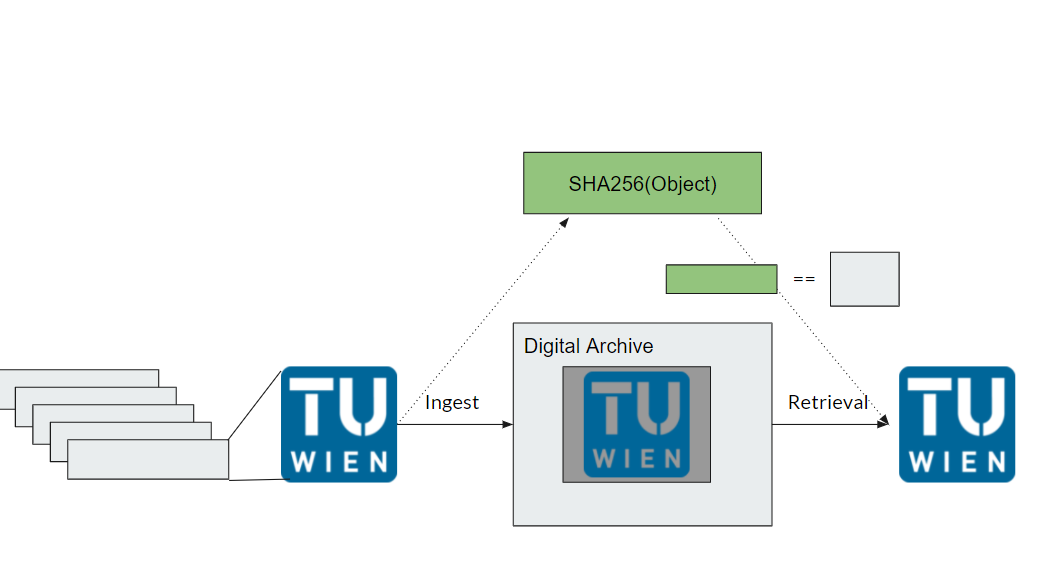
\includegraphics[width=0.75\textwidth]{lifecycle.png}
\end{figure}
\section{Implementation}
\label{sec:implementation}
The fixity storage presented in this thesis is implemented in Solidity, a programming language designed for the EVM, see Section \ref{sec:evm}.
The basic functionality of the smart contract, as described in Section \ref{sec:approach} can be seen in the source code presented in Listing \ref{lst:fixity-storage}
\begin{lstlisting}[language=Solidity,caption={MVP source code of the fixity storage deployed on the Ropsten test network \url{https://Ropsten.etherscan.io/address/0x0243c7aa552730E8C6F7ED25A480a7C0c88a70f0}},label=lst:fixity-storage]
// SPDX-License-Identifier: MIT
pragma solidity >=0.4.22 <0.9.0;

contract FixityStorage {
  mapping(uint32=>bytes32) pools;
  address creator;

  constructor()public{
    creator = msg.sender;
  }

  function getPoolHash(uint32 poolId) public view returns(bytes32) {
      return pools[poolId];
  }

  function setPoolHash(uint32 poolId, bytes32 poolHash) public {
    require(msg.sender==creator);
    pools[poolId]=poolHash;
  }
}
\end{lstlisting}
where \textit{getPoolHash(uint32 poolId)} implements a read function; \textit{setPoolHash(uint32 poolId,bytes32 poolHash)} implements create and update function. The mapping type is native in solidity which implements a hash map consisting of a key and a value, where in this case the key is an integer representing the \textit{poolId} and the value is a \textit{bytes32} object representing the SHA256 root hash of the pool. The \textit{poolId} is the reference to the local pool in the digital archive, with which fixity information can be retrieved for a certain pool from the contract. The solidity language presents a convenient  method to prevent unauthorized calls to the setPoolHash() method, which is \textit{require(msg.sender==creator)}. The native method \textit{require} is a "guard" function which improves the readability of the smart contract code which fires a REVERT instruction if the condition is not met. The condition in this case is, that only the creator, which is set in the constructor, of the fixity storage is able to create and alter the information stored on the blockchain.

\section{Deployment}
I utilized truffle\footnote{\url{https://trufflesuite.com/index.html}} to run my deployment of the smart contract, it brings built-in smart contract compilation, linking, deployment and binary management with automated contract testing. The reasoning behind my decision is that, truffle has all the tools needed to implement a smart contract in one package and therefore reduced complexity in the development process. In the first iteration of the development process, I used the graphical user-interface Ganache\footnote{\url{https://trufflesuite.com/ganache/index.html}} to get a better feeling for the Ethereum blockchain, see Figure \ref{fig:ganache}.
\begin{figure}[h]
  \caption{Ganache, an interactive user interface for the Ethereum blockchain.}
  \label{fig:ganache}
    \centering
    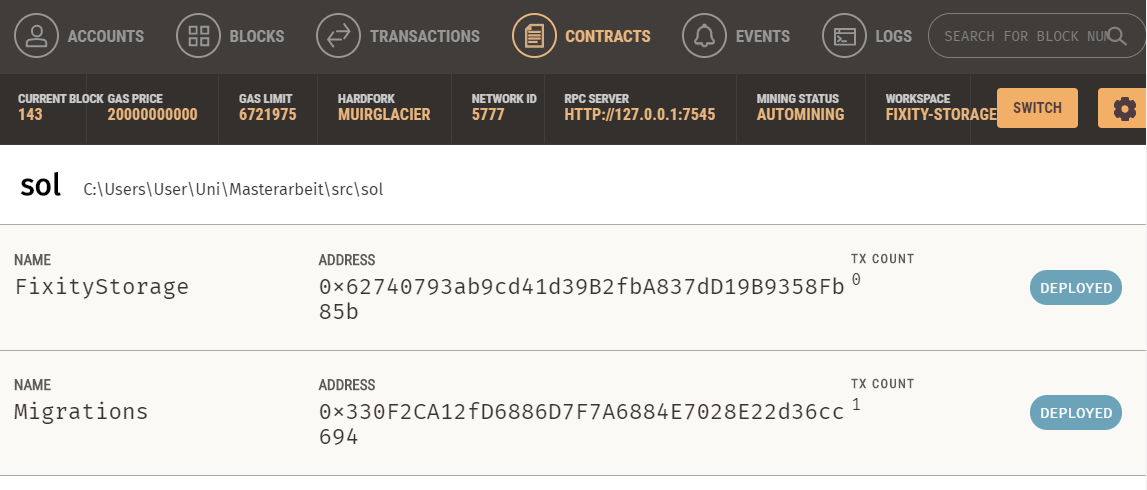
\includegraphics[width=0.7\textwidth]{ganache.png}
\end{figure}
It allows you to click through your smart contract and look at the state variables or functions to validate that your smart contract was successfully deployed. Ganache has a massive disadvantage when doing high throughput computing, it seems that it is not suited to withstand 10000 transactions built in a python for loop. Therefore, I only used the GUI it in the beginning of the experiment where I only persisted about 10 objects at a time without problems. For high throughput computing, truffle offers a command line tool to interact with the blockchain. The command line tool was resistant and showed no weakness when persisting 10000 objects.
Truffle also allows to config other networks, e.g. the Ropsten test network, which can be defined as a parameter in the deployment process. The deployment requires to have some ETH token in your account to pay the miner to integrate your smart contract in a block. 
Truffle offers some utility regarding automated deployment, which are migrations. Migrations are JavaScript files, which are responsible for staging the deployment tasks and running deployment scripts. I used the migrations feature in order to interact with various Ethereum networks, in my case the Ropsten test network and a local test environment. The migrations feature requires to have a smart contract deployed on the blockchain, which causes additional cost (191943 gas) to the fixity storage, therefore I have decided not to use the migrations feature, as it is controversial in the community and seen as unnecessary traffic and cost\footnote{\url{https://github.com/trufflesuite/truffle/issues/503}}.
The deployment cost of the smart contract can be calculated as follows:
\begin{equation}\label{eq:create-cost}
  \begin{split}
      C_{deployment} & = transaction + txcreate + codedeposit + txdatanonzero + txdatazero \\
      & = 21000 + 32000 + 200 * 832 + 226 * 4 + 800 * 16 \\
      & = 233104
  \end{split}
\end{equation}
where $transaction$ is the base cost for a transaction; $txcreate$ is the operation used to create a smart contract; $codedeposit$ is the gas cost for each byte of the runtime bytecode of the smart contract, which is 832 bytes and can be seen in the Input Data field of the transaction on Etherscan\footnote{\url{https://ropsten.etherscan.io/tx/0x844f76cfff6e00f29487f6fe3c99d8a69eab576e7c190e5b392745b48924a1f6}}
\textit{$G_{txdatanonzero}$} is 16 gas for each non-zero byte in the compiled bytecode of a transaction;\textit{$G_{txdatazero}$} is 4 gas for each non-zero byte in the compiled bytecode of a transaction; and \textit{$Contract_{bytesize}$} is the size of the compiled bytecode of the contract, see Section \ref{sec:costs} for the exact gas amount for each transaction.
The amount of gas consumed by the deployment of the decentralized fixity storage is 166079 gas on the Ropsten testnet, the transaction used to deploy the contract can be found on Etherscan\footnote{\url{https://ropsten.etherscan.io/tx/0xf383c4bf0a5c32dd3369b02f68fd4e4400ef59343ad472bc96a28827f32c9abb}}, where additional information can be read. The address of the smart contract is \textit{0x0243c7aa552730E8C6F7ED25A480a7C0c88a70f0}.
\section{Authorized Access}
In solidity one can require a certain address to access a function, the keyword requires can be used  so that a transaction from an unknown address can be reverted and only the owner of the creator address can update the mapped SHA256 values in the smart contract. An interesting topic is also how the private key in the archive may be managed, which is not part of this thesis, but something like a multisignature wallet may be used to split the responsibility of the owner address in the contract. Since the entity which controls the private key of the smart contract is able to perform update operations which can lead to unwanted actions. In the worst case, an unwanted action may be ignored, since the older value is not deleted on the blockchain. Therefore, the key user management of the smart contract can be used as a next step in further research. For this thesis I assume that the private key is well managed and each transaction coming from the master address is legit.
\section{Cost of interacting with the fixity storage}\label{sec:cost-interating}
The cost of interacting with the fixity storage depends on the desired action. There are three different way to interact with the contract: (1) create a new entry (2) update an existing entry and (3) read an entry.
The cost of a transaction, which invokes the setPoolHash function and ultimately stores 256 bit on the blockchain can be calculated with Equation \ref{eq:tx-cost}
\begin{equation}\label{eq:tx-cost}
    \begin{split}
        C_{setPoolHash} & = gasAmount * gasPrice * ethPrice \\ 
        & = 42368 * 0.00000005 * 4000
    \end{split}
\end{equation}
which results in \$8.47 on average for an ETH price of \$4000.
The $gasAmount$ in Equation \ref{eq:tx-cost} can be calculated as follows:
\begin{equation}\label{eq:tx-data}
  \begin{split}
    gasAmount & = transaction + sset + txdatazero + txdatanonzero \\
     & = 21000 + 20000 + 16 * 68 + 4 * 70  \\
     & = 42368
  \end{split}
\end{equation}
where $txdatazero$ is the number of zeros in the transaction data and $txdatanonzero$ is the amount of non-zero bytes in the transaction data. The transaction data for Equation \ref{eq:tx-data} can be found here in the Input Data field of the transaction on Etherscan\footnote{\url{https://ropsten.etherscan.io/tx/0x8839e03f0143bad34060fa909c35d30f2edb22dd4fdac0264de8ae84176eb1ea}}.
The cost for updating an existing entry can be calculated in the same way as for creating ones, with the difference that the costly $sset$ operation can be spared and therefore updates costs 20000 gas less than creates.
Reading an entry is free of charge, since no state changes has to be forwarded to the blockchain.
To explain the cost of the non-zero and zero bytes can be explained by looking the following Input Data

\hash{0x178d292900000000000000000000000000000000000000000000000000000000000000001760d27083f6e2d1c46a65938c03a0c52dccf55cb4eb68a720e6efe3a8851f78}

where zero and nonzero bytes are counted and multiplied by their respective gas cost, which in this example is $txdatazero+txdatanonzero = 4 * 70 + 16 * 68 = 1368 $. The amount of non-zero bytes can be interpreted as the amount of effort given to the network.

\section{Proof of Concept}\label{sec:poc}
The proof of concept is written in Python in form of a Jupyter Notebook. It can be found on GitHub \url{https://github.com/metsch/masterthesis/blob/main/src/py/poc_ropsten.ipynb}. With Python's Web3.py I get the contract from the blockchain and extract its functions setPoolHash and getPoolHash. For the live experiment on the Ropsten test network I have initialized 100 digital objects, in form of SHA256 values, with a prevalence rate of 0.1 (or 10\%). The less amount of objects in the live experiment is due to the fact, that the Ropsten ETH token is hard to get, since the most relevant publicly available faucets are drained out and the ones available have a rate of only 0.1 ETH per day, as I explained in Section \ref{sec:test-nets}. I computed the optimal pool size k for N=100 and p=0.1 with Equation \ref{eq:poolsize} and created $\lceil N/k \rceil$ pools. Each pool is assigned an ID and has an array of objects, from which a hash list is formed, and the resulting root hash is stored. 
Before uploading the pools on to the blockchain, I estimated the gas cost for a single transaction in order to set the gas limit to avoid overpaid transactions. I utilized Equation \ref{eq:tx-data} and added 20\% in order guarantee that the transaction is not underpaid, since the result of Equation \ref{eq:tx-data} is the exact gas amount and may be reverted.
At the time of the experiment, the gas price was 86.11 gwei which is 0,0000000896 ETH, resulting in \$15.18 for a setPoolHash transaction calculated with Equation \ref{eq:tx-cost} with an ETH price of \$4000. Admitted, this gas price is really high, usually the gas price is about 40 gwei. 
For each pool, 25 in total, I uploaded each root hash on to the blockchain and waited for the transaction to finish and run some tests to see if the transactions were successful.
After uploading the root hashes, I artificially corrupted the objects in the archive with a Bernoulli trial where an object gets corrupted if a random number between 0 and 1 is below p=0.1. At last, I repaired the archive by checking the local pools with the ones on the blockchain, and if the pool hashes did match the pool is seen as uncorrupted. Where the pools with non-matching hashes got replaced by copies of the objects.
To sum it up, the cost for the live experiment was for 25 writing transactions 0.11204969029 ETH (\$448) and 8 data-scrubbing operations resulting in 33 total operations. Whereas, with an individual testing strategy the amount of writing transactions would have been 100 and estimated 10 data-scrubbing operations. The experiment showed no weakness in throughput, where 25 transactions were uploaded in an instant and mined in less than 2 minutes

\section{Wrap Up}
In this Chapter I have presented the various forms of fixity information with their respective advantages and disadvantages together with my reasoning on why I have decided to utilize SHA256 cryptographic hashes. I have also presented various storage-media for fixity information and why it is so important that these storages guarantee for immutability in regard to history forgery. The interactions with the fixity storage are tested in an experimental environment, presented in the following section \ref{sec:poc}.